
\documentclass[12pt]{article}
\usepackage{graphics,amssymb,amsmath}

\usepackage[slovak]{babel}
\usepackage[utf8]{inputenc}
\usepackage[IL2]{fontenc}

\usepackage{multicol}
\usepackage{mathtools}

\pagestyle{empty}
\setlength\textwidth{170mm}
\setlength\textheight{265mm}
\addtolength\oddsidemargin{-20mm}
\addtolength\topmargin{-20mm}
\setlength{\parindent}{1pt}
\setlength{\parskip}{10pt}
\newcount\pocet
\pocet = 1
\def\pr{{\bf \the \pocet .\ \global\advance\pocet by 1}}

\newcommand{\g}{ \dots \dots \dots \dots \dots \ }
\newcommand{\gu}{ \dots \dots \ }
\newcommand{\gr}{\dotfill \ }

\begin{document}

\newenvironment{itemize*}
{\begin{itemize}
\setlength{\itemsep}{0pt}
\setlength{\parskip}{0pt}}
{\end{itemize}}

\newenvironment{enumerate*}
{\begin{enumerate}
\setlength{\itemsep}{0pt}
\setlength{\parskip}{0pt}}
{\end{enumerate}}


\phantom{a}

\centerline{\textbf{\Large Matematika I}}
\smallskip
\centerline{05. január 2020}
\centerline{9:00}
\vskip0.5cm

\centerline{\bf  Meno a priezvisko: \gr Podpis: \gr}
\vskip0.5cm
\centerline{\bf  Ročník: \gr študijný program: \gr}
\vskip0.5cm

\medskip

\pr (7b) Daná je všeobecná rovnica kužeľosečky
$9x^2+4y^2-1 = 0$.

\medskip

\noindent
\textbf{Doplňte:}
\begin{enumerate}
\item[a)] (2b) Kanonická rovnica (rovnica v štandardnom tvare) kužeľosečky je\gr
\item[b)] (1b) Typ kužeľosečky je \gr
\item[c)] (3b) Napíšte, ak existujú
\begin{itemize}
\item[$c_1$)] súradnice stredu kužeľosečky: \gr
\item[$c_2$)] súradnice ohniska resp. ohnísk kužeľosečky: \gr
\item[$c_3$)] súradnice vrcholu resp. vrcholov kužeľosečky: \gr
\end{itemize}
\item[d)] (1b) Znázornite kužeľosečku a v náčrte popíšte jej charakteristické prvky.
\end{enumerate}

\newpage

\pr (2b) Vyberte funkciu, ktorej definičný obor je znázornený na obrázku.
\begin{multicols}{2}
\noindent
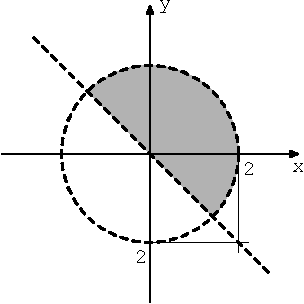
\includegraphics{kruznica2.pdf}

\noindent
\begin{itemize}
\item[a)] $\displaystyle f(x,y)= \ln{(x^2+y^2-1)}+\sqrt{4-x^2-y^2}$
\item[b)] $\displaystyle f(x,y)= \frac{\ln{(4-x^2-y^2)}}{\sqrt{x^2+y^2-1}}$
\item[c)] $\displaystyle f(x,y)= \frac{\sqrt{x^2+y^2-1}}{\ln{(4-x^2-y^2)}}$
\item[d)] $\displaystyle f(x,y)= \sqrt{x^2+y^2-1}-\ln(4-x^2-y^2)$
\end{itemize}
\end{multicols}

\pr (6b) Vypočítajte
$$\iint\limits_{M}{y} \ \mathrm{d}x \mathrm{d}y,$$
kde množina $M$ je mnohouholník s vrcholmi
$A=[-1, -1]$,
$B=[1, -1]$,
$C=[4, 3]$,
$D=[-4, 3]$.

\begin{enumerate}
\item[]\textbf{Výsledok:}\gr
\end{enumerate}

\pr (4b) Toto je príklad typu A

text text text \\ \\

\pr (5b) Toto je príklad typu B

text text text \\ \\

\pr (6b) Toto je príklad typu D

text text text \\ \\

\pr (7b) Toto je príklad typu F

text text text \\ \\

\pr (8b) Toto je príklad typu A

text text text \\ \\

\pr (9b) Toto je príklad typu C

text text text \\ \\


\end{document}